\documentclass[newPxFont,numfooter,sectionpages]{beamer}
\usepackage[utf8]{inputenc}
\usetheme{sthlm}
\usepackage[round]{natbib}
\bibliographystyle{plainnat}
\usepackage{amsmath}
\usepackage{amssymb}
\usepackage{amsthm}
\usepackage{dsfont}
\usepackage{hyperref}
\usepackage{multirow}
\usepackage{color}
\usepackage{tikz}
\usepackage{graphicx}
\usepackage{setspace}
\usepackage{bigints}
\usepackage{algorithm2e}
\usepackage{float}
\usepackage{lscape}
\usepackage{rotating}
\usepackage{longtable}
\usepackage[normalem]{ulem}
\hypersetup{
    colorlinks=true,
    linkcolor=black,
    filecolor=magenta,
    urlcolor=blue,
    citecolor=black,
}

\newcommand{\indep}{\mathrel{\text{\scalebox{1.07}{$\perp\mkern-10mu\perp$}}}}
\DeclareMathOperator*{\argmin}{arg\,min}
\DeclareMathOperator*{\argmax}{arg\,max}
\newcommand{\E}{\mathbb{E}}
\newcommand{\V}{\mathbb{V}}
\newcommand{\I}{\mathbb{I}}
\newcommand{\com}[1]{&&\mbox{(#1)}}
\newcommand{\bt}{\mathbf{t}}
\newcommand{\bT}{\mathbf{T}}
\newcommand{\Gni}{G_{\mathcal{N}_i^\bt}}
\newcommand{\Gnj}{G_{\mathcal{N}_j^\bt}}
\newcommand{\btheta}{\boldsymbol{\phi}}

\title{Almost-Matching-Exactly for Treatment Effect Estimation under Network Interference}
\subtitle{}
\author{Usaid Awan, Marco Morucci, Vittorio Orlandi}

%\institute{Duke University}
\date{}
\begin{document}
\setbeamercolor{background canvas}{bg=dukeBlue}
\setbeamercolor{title}{fg=white} \setbeamercolor{subtitle}{fg=white}
\setbeamercolor{institute}{fg=white}
\setbeamercolor{author}{fg=white}
\setbeamercolor{normal text}{fg=white}
\maketitle

\setbeamercolor{background canvas}{bg=white}
\setbeamercolor{frametitle}{bg=dukeBlue}
\setbeamercolor{normal text}{fg=sthlmDarkGrey, bg=sthlmGrey}

\begin{frame}{Setting - Causal Inference}
\begin{itemize}
  \item We have $i=1, \dots, n$ experimental units
  \item Treatment $t_i \in \{0, 1\}$ with $\bt \in \{0, 1\}^n$ is a binary vector with the treatment level of every unit.
  \item Potential outcomes $Y_i(t_i, \bt)$ are random variables and depend on both treatment of unit $i$ (1st argument), and treatment of \textbf{all other units} (2nd argument).
  \item Observed treatment $\bT \in \{0, 1\}^n$ is assigned \textbf{uniformly at random}.
  \item Observed outcome: $Y_i = T_iY(1, \bT) + (1-T_i)Y_i(0, \bT)$
  \begin{itemize}
    \item Since treatment is randomized: $\E[Y_i|\bT = \bt, T_i = t] = \E[Y_i(t, \bT)]$ (Ignorability).
  \end{itemize}
  \item Units are connected in a network, $G$, in which unit $i$'s \textbf{neighborhood subgraph} is $\Gni$.
\end{itemize}
\end{frame}

\begin{frame}{The Problem: No SUTVA!}
Usually we assume that \textit{units' treatments don't influence other units' outcomes}, but we can't do that here because our units are connected in a network:
\begin{center}
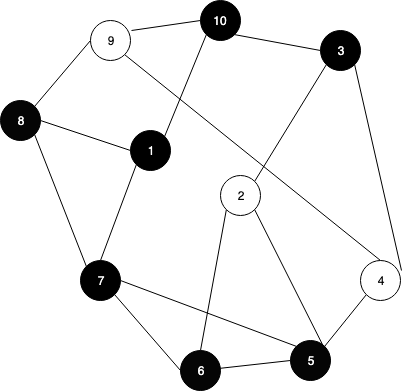
\includegraphics[height=1.8in]{graph1.png}
\end{center}
It could be that the treatment assigned to $j$ influences the outcome of $i$ through their connection in the network.
\end{frame}

\begin{frame}{Similar Graphs Carry Similar Interference}
\begin{alertblock}{Idea}
What if the amount of interference experienced by a unit depended on the \textit{shape} of its treated neighborhood subgraph?
\end{alertblock}
\begin{center}
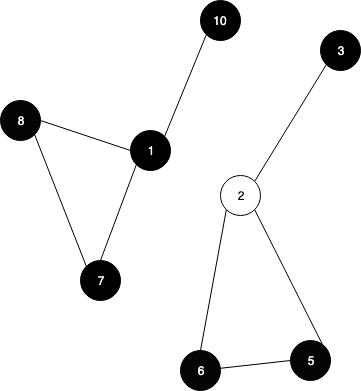
\includegraphics[height=1.5in]{graph2.png}
\end{center}
Then, in expectation, two units with the same treated neighborhood graph will respond similarly to the treatment. \\
\textbf{We can use this idea to do matching to reduce interference.}
\end{frame}

\begin{frame}{Assumptions}
\begin{enumerate}
  \item Outcome model: $Y_i = \alpha + t_i\tau_i + f(\Gni) + \epsilon_i$
  \begin{itemize}
    \item $f$ is some interference function dependent on $\Gni$, the \textbf{treated neighborhood subgraph} of unit $i$.
  \end{itemize}
  \item $\E[\epsilon_i] = 0$
    \begin{itemize}
    \item Ignorability
  \end{itemize}
  \item $|\E[f(g)] - \E[f(h)]| \leq K_1||g - h||$
  \begin{itemize}
    \item The more similar the neighborhood graphs of $i$ and $j$, the more similar the amount of interference they receive.
    \item Together with (1), this assumption encodes a version of SANASIA (Airoldi and Sussman, 2018) conditional on unit's neighborhood subgraphs.
  \end{itemize}
\end{enumerate}
\begin{alertblock}{Problem}
How do we represent similarity between neighborhood graphs?
\end{alertblock}
\end{frame}
\begin{frame}{The Exponential Random Graph Model for Networks}
A model in which networks are fully described by a set of statistics, like subgraph counts and nodal attributes. 
\begin{itemize}
  \item $\Pr(\Gni = g) = \frac{exp(\btheta^TS(g))}{\sum_{h \in \mathcal{G}} exp{\btheta^TS(h)}}$
  \item Here $S(g)$ is a function that takes a network and outputs a vector of network statistics
  \item Two graphs with the same values for the statistics of interest have the same probability
\end{itemize}
Here we focus on \textbf{subgraph counts} as statistics, i.e., how many of each subgraph type does each unit have in its treated neighborhood graph.
\end{frame}
\begin{frame}{Putting It All Together}
If we make an additional assumption$^*$, that the network statistics represent correctly each unit's neighborhood graphs, i.e.:
\begin{align*}
|\E[Y_i(t, \bt)|S(\Gni)=\mathbf{a}] - \E[Y_j(t, \bt)|S(\Gnj)=\mathbf{b}]| \\ \leq K_2||\mathbf{a} - \mathbf{b}||
\end{align*}
Then if we match units with similar neighborhood graphs, we will reduce bias and eventually recover the correct treatment effect:
\begin{align*}
\E[Y_i(t, \bt)|S(\Gni)=\mathbf{a}] = \E[Y_j(t, \bt)|S(\Gnj)=\mathbf{a}]\quad \forall i, j
\end{align*}
$*$ \small{Unclear whether we have to make this assumption or whether it follows from ERGM. }
\end{frame}
\begin{frame}{$\cdot$AME-Networks}
\begin{alertblock}{Problem \#2}
How do we choose which subgraph we should use to represent the treated neighborhood graphs of our units?
\end{alertblock}
\textbf{Use FLAME to choose which subgraphs to count!}
\begin{enumerate}
  \item Count all possible subgraphs that are in each unit's treated neighborhood graph
  \item These are likely a lot and it's unlikely that many units will have the exact same counts
  \item Use FLAME to make almost-exact matches on subgraph counts 
\end{enumerate}
\end{frame}
\begin{frame}{A Small Change to FLAME}
We know from our theoretical setup that network statistics should do two things well:
\begin{enumerate}
  \item Predict the \textbf{outcomes}
  \item Predict the \textbf{network}
\end{enumerate}
Therefore, it makes sense that the FLAME objective should trade-off between these things:
\begin{align*}
{\tt PE} &= \sum_{t = 0}^1\argmin_{f \in \mathcal{F}}\frac{1}{n}\sum_{i = 1}^n(Y_i - f(S(\Gni)))^2\\
         &- C\argmax_{\btheta \in \mathbb{R}^{|S|_0}}\underbrace{\frac{1}{n}\sum_{i=1}^n\btheta^TS(\Gni) - \log\left(\sum_{g \in \mathcal{G}} \btheta^TS(g)\right)}_{\text{ERGM log-likelihood}}
\end{align*}
\end{frame}
\begin{frame}{(OLD) Simulation Results}
\centering
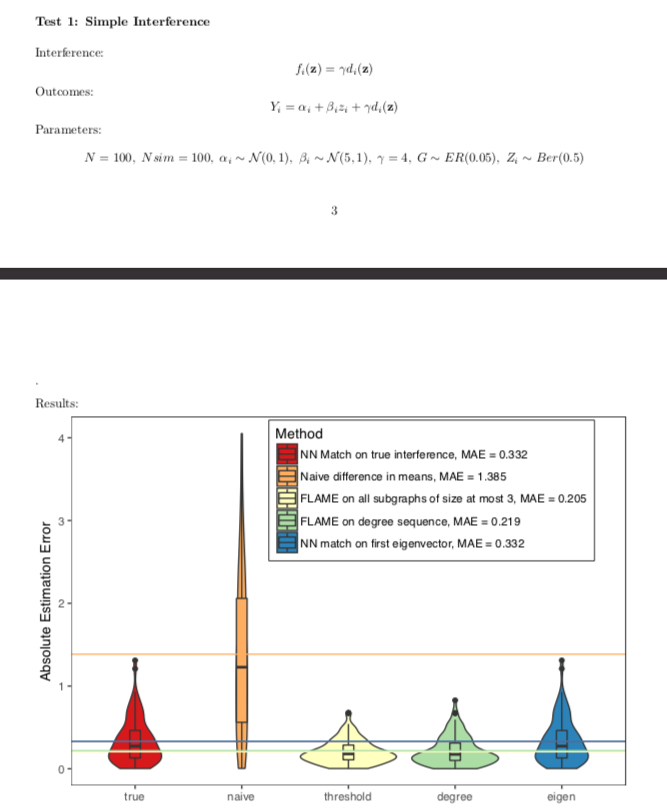
\includegraphics[height=3in]{simple.png}
\end{frame}
\begin{frame}{(OLD) Simulation Results}
\centering
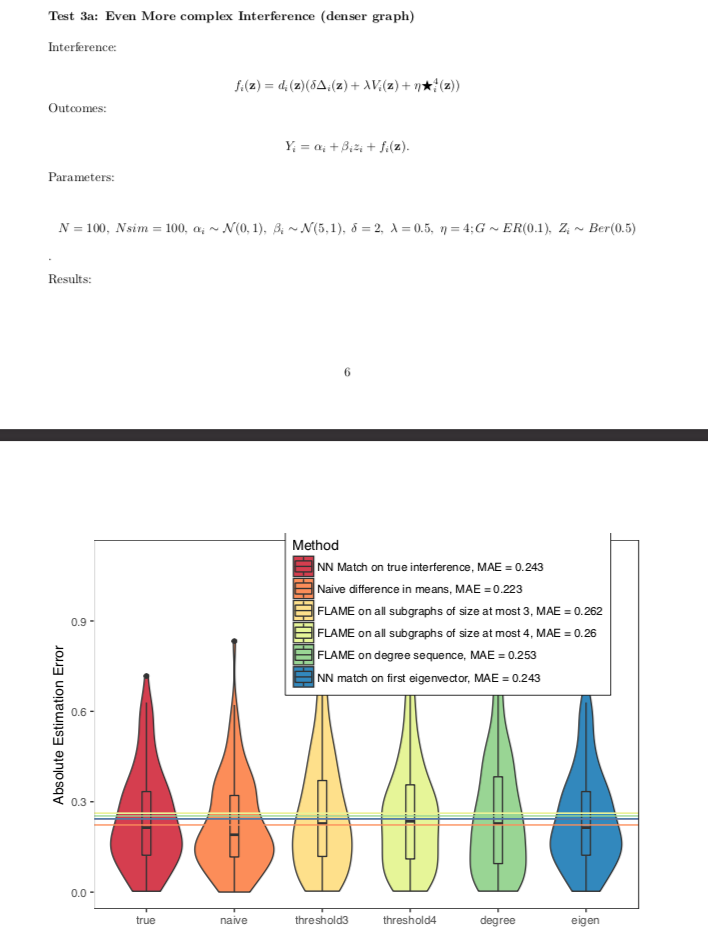
\includegraphics[height=3in]{even_more_complex.png}
\end{frame}
\begin{frame}{(OLD) Simulation Results}
\centering
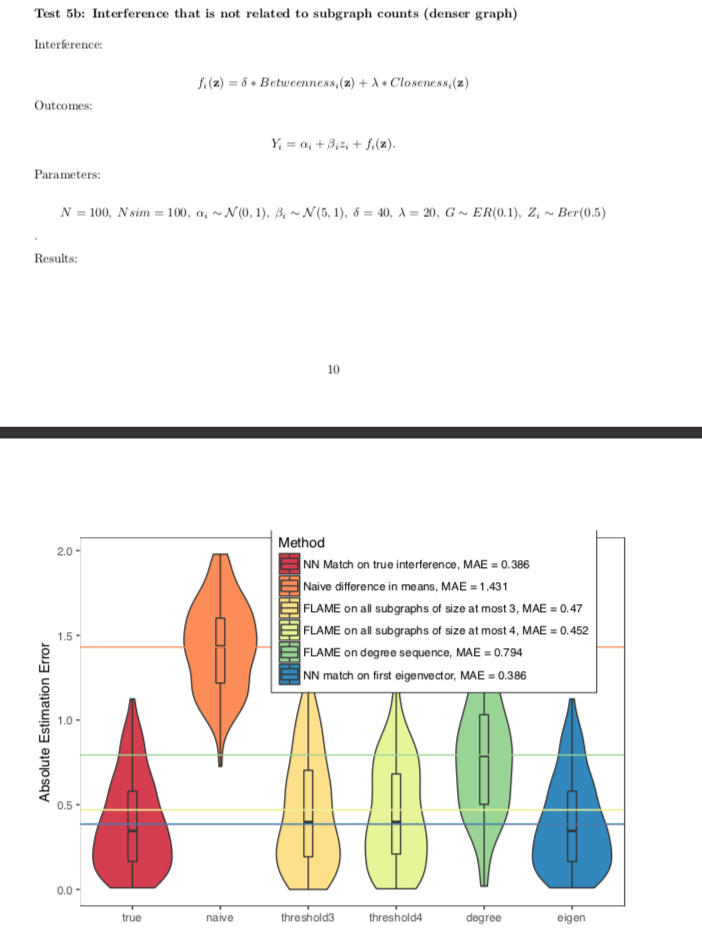
\includegraphics[height=3in]{unrelated_dense.png}
\end{frame}
\begin{frame}{Bias Bound for oracle AME}
As a preliminary result we can say that, under all the assumptions made before, with the true value of $\btheta$ and $S$ known, and if we choose a match for unit $i$ with treated neighborhood graph $g$ such that:
\begin{align*}
j \in {\tt MG(g)} \text{ if } j \in \argmin_{j = 1, \dots, n, T_j = 0} |\btheta^TS(g) - \btheta^TS(\Gnj)|,
\end{align*}
then the bias for the CATT of $i$ can be upper bounded by:
\begin{align*}
|\E[Y_i - Y_j] - \tau_i| &\leq K_1\sum_{h \in \mathcal{G}}|\btheta^TS(g) - \btheta^TS(h)|\frac{exp(\btheta^TS(h))}{\sum_{\ell \in \mathcal{G}}exp(\btheta^TS(\ell))}\\
&\times\left[\sum_{d = S(g) - |S(g) - S(h)|}^{S(g) + |S(g) - S(h)|}\frac{D_{\btheta, S}(d)exp(d)}{\sum_{\ell \in \mathcal{G}}exp(\btheta^TS(\ell))}\right]^{n - 1}
\end{align*}
\end{frame}
\begin{frame}{Plan: We Want to Hit the October 8 AISTATS Deadline}
\begin{enumerate}
  \item We need to implement the revised $\tt PE$ function
  \item We need to redo the simulations
  \item More theory? Statements on how well the subgraph count can ``encode'' a given graph would be nice
  \item Find a good application
  \item Write!
\end{enumerate}
\end{frame}
\end{document}




